\documentclass[12pt]{article}
\usepackage[spanish]{babel}
\usepackage[utf8]{inputenc}
\usepackage[T1]{fontenc}
\usepackage{FiraSans}
\usepackage{amsmath}
\usepackage{graphicx}
\usepackage{float}
\usepackage{subfig}
\usepackage{array}
\renewcommand{\familydefault}{\sfdefault}
\renewcommand{\arraystretch}{1.1}

\begin{document}

\begin{titlepage}
\newcommand{\HRule}{\rule{\linewidth}{0.5mm}} 
\center


\includegraphics[scale=0.4]{images/logo-usm.png}\\
\vspace{0.6cm}
\textsc{\large INF480}\\[0.5cm] % Minor heading such as course title
\textsc{\Large Redes Complejas}\\[0.5cm] % Major heading such as course name

\HRule \\[0.4cm]
{ \huge \bfseries Tarea 2}\\[0.4cm] % Title of your document
\HRule \\[1.5cm]
 
\begin{minipage}{0.8\textwidth}
\begin{center} \large
Florencia Ramírez, ROL: 202073522-0\\
Sofía Riquelme, ROL: 202073615-4
\end{center}

\end{minipage}\\[2cm]

\vfill 

\end{titlepage}
\begin{enumerate}
    \item La matriz laplaciana del grafo es la siguiente:

    \[
    \begin{bmatrix}
        2 & -1 & -1 &  0 &  0 &  0 &  0 \\
        -1 &  2 & -1 &  0 &  0 &  0 &  0 \\
        -1 & -1 &  3 & -1 &  0 &  0 &  0 \\
        0 &  0 & -1 &  3 & -1 & -1 &  0 \\
        0 &  0 &  0 & -1 &  2 & -1 &  0 \\
        0 &  0 &  0 & -1 & -1 &  3 & -1 \\
        0 &  0 &  0 &  0 &  0 & -1 &  1
    \end{bmatrix}
    \]

    El valor de Fiedler para esta matriz es $0.34032095848177074$ y el vector propio asociado es el siguiente: 
    \[
    \begin{bmatrix}
         -0.46724728 \\
         -0.46724728 \\
         -0.30823323 \\
          0.11469308 \\
          0.27370712 \\
          0.33957289 \\
          0.5147547 
    \end{bmatrix}
    \]

    Luego, el gráfico de la red con sus comunidades es el siguiente:
    \begin{figure}[H]
        \begin{center}
            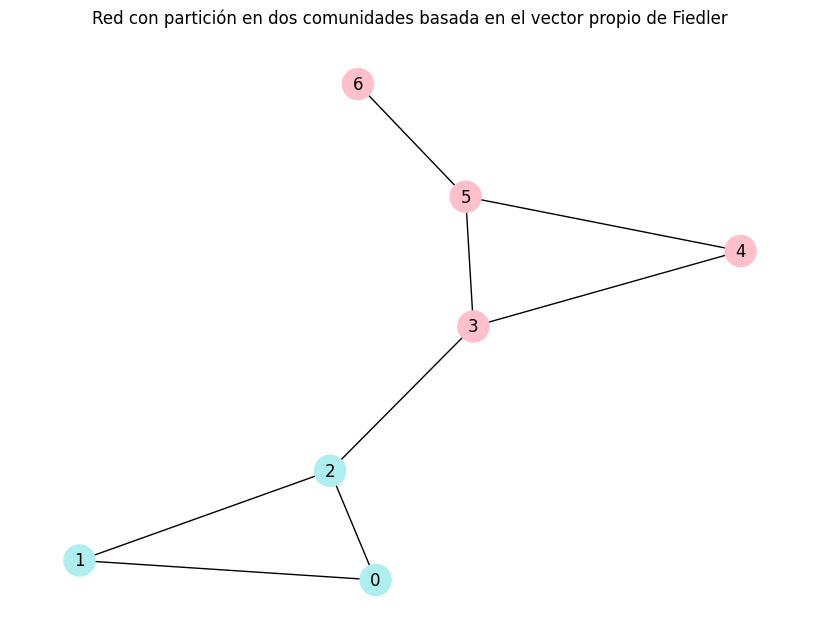
\includegraphics[scale=0.4]{images/grafico_red.png}
        \end{center}
        \caption{Gráfico de red}
        \label{fig:graph}
    \end{figure}

    \item 
    \begin{enumerate}
        \item Para que $P$ sea una distribución de probabilidad, debe ocurrir lo siguiente:
        $$\sum_{k=0}^{\infty}  P(k) = 1 $$
        Luego, dado que $P(k) = C \times \alpha ^k$, se tiene que 
        $$\sum_{k=0}^{\infty} C \alpha ^k= 1 $$
        Esto es una serie geométrica. La serie geométrica infinita $( \sum_{k=0}^{\infty} \alpha^k )$ converge a $( \frac{1}{1-\alpha} )$ siempre que $( |\alpha| < 1 )$. Por lo tanto,
        $$ \sum_{k=0}^{\infty} C \alpha ^k= C \left(\frac{1}{1-\alpha}\right) = 1 $$
        Despejando $C$:
        $$C = 1-\alpha$$

        \item La función generadora de un grafo, es $G_p(x) = \sum p_k x^k$. Como se vio en el ítem anterior, tenemos que $P(k) = C\alpha^k$ y $C = 1-\alpha$. Si sustituimos, se tiene que: 
        $$G(x) = \sum_{k=0}^{\infty}(1-\alpha)\alpha^k x^k$$ 
        $$G(x) = (1-\alpha)\sum_{k=0}^{\infty}(\alpha x)^k$$ 
        Utilizando la misma convergencia de series geométricas, se tiene que la expresión generadora para la distribución de grados es:
        $$G(x) = (1-\alpha)\left(\frac{1}{1-\alpha x}\right)$$

        \item Al solamente tener información de la distribución de grados, se tiene una componente gigante en el grafo cuando se cumple:
        $$\sum_{i=0}^{\infty} i (i - 2) P(i) > 0$$

        Sustituimos $P(k) = C\alpha^k$ y $C = 1-\alpha$ en la expresión:
        $$\sum i_{i=0}^{\infty} (i - 2) (1 - \alpha) \alpha^{i} > 0$$
        $$(1 - \alpha) \sum_{i=0}^{\infty} i (i - 2) \alpha^{i} > 0$$
        $$(1 - \alpha) (\sum_{i=0}^{\infty} i^{2} \alpha^{i} - 2 \sum_{i=0}^{\infty} i \alpha^{i}) > 0$$
        $$(1 - \alpha) (\frac{\alpha (1 + \alpha)}{(1-\alpha)^{3}} - 2 \frac{\alpha}{(1-\alpha)^{2}}) > 0$$
        $$(1 - \alpha) (\frac{3\alpha^{2} - \alpha}{(1-\alpha)^{3}}) > 0$$
        $$\frac{3\alpha^{2} - \alpha}{(1-\alpha)^{2}} > 0$$
        
        Con lo cual se puede despejar $\alpha$, obteniendo que:
        $$\frac{3\alpha^{2} - \alpha}{(1-\alpha)^{2}} > 0$$
        $$3\alpha^{2} - \alpha > 0$$
        $$\alpha (3\alpha - 1)> 0$$
        $$\alpha > \frac{1}{3}$$

        Finalmente como tenemos $0 < \alpha < 1$, para que exista una componente gigante en el grafo se tiene que cumplir que $\frac{1}{3} < \alpha < 1$.
    \end{enumerate}

    \item Al hacer las eliminaciones se obtuvieron los siguientes resultados:
    \begin{table}[H]
        \footnotesize
        \centering
        \begin{tabular}{|l|c|c|c|c|}
            \hline
            \textbf{Red} & \textbf{Nodos Iniciales} & \textbf{Aleatorio} & \textbf{Por Grado} & \textbf{Por Betweenness} \\
            \hline
            Piratas & $795$ & $32.08\%$ & $3.02\%$ & $3.14\%$ \\
            \hline
            Delfines & $62$ & $38.71\%$ & $24.19\%$ & $12.90\%$ \\
            \hline
            ER Piratas & $795$ & $29.94\%$ & $8.18\%$ & $5.16\%$ \\
            \hline
            ER Delfines & $62$ & $48.39\%$ & $30.65\%$ & $29.03\%$ \\
            \hline
        \end{tabular}
        \caption{Resumen de Eliminaciones en Diferentes Redes}
        \label{tabla:resumen_eliminaciones}
    \end{table}
     Se puede observar que en el caso de la red Piratas (la original y la ER), al eliminar por grado y por betweenness se requiere un bajo porcentaje de nodos para que la componente gigante baje considerablemente su tamaño. Sin embargo, en las redes de Delfines, en todos los casos se requiere eliminar un porcentaje no menor. 
     Esto sugiere que la red de piratas es extremadamente vulnerable a ataques dirigidos, lo cual se puede deber a que tiene una estructura centralizada, a diferencia de la red de delfines. Asimismo las redes ER, muestran una mayor fragilidad por su estructura más homogénea.

    \item Luego de calcular la modularidad promedio $Q^{d}(p)$ para las dos posibles particiones se obtuvieron los siguientes resultados:
    
    \begin{table}[H]
        \centering
        \begin{tabular}{|c|c|c|}
            \hline
            \textbf{$p$} & \textbf{$Q_{B}^{d}$} & \textbf{$Q_{C}^{d}$} \\ \hline
            $0.0$ & $0.12800588$ & $0.00190496$ \\ \hline
            $0.1$ & $0.08123612$ & $0.00073970$ \\ \hline
            $0.2$ & $0.04913890$ & $0.00231686$ \\ \hline
            $0.3$ & $0.02125331$ & $0.00156286$ \\ \hline  
            $0.4$ & $0.00902243$ & $0.00217117$ \\ \hline
            $0.5$ & $0.00398928$ & $0.00112336$ \\ \hline
            $0.6$ & $0.00727439$ & $0.00381207$ \\ \hline
            $0.7$ & $0.02271023$ & $0.00177777$ \\ \hline
            $0.8$ & $0.04808281$ & $0.00401861$ \\ \hline
            $0.9$ & $0.08286395$ & $0.00197586$ \\ \hline
            $1.0$ & $0.12718032$ & $0.00194545$ \\ \hline
        \end{tabular}
        \caption{Modularidad dirigida para distintos valores de $p$}
        \label{tab:modularidad}
    \end{table}
    
    Se presenta un gráfico mostrando la relación entre estos valores obtenidos para la modularidad en función de $p$:

    \begin{figure}[H]
        \centering
        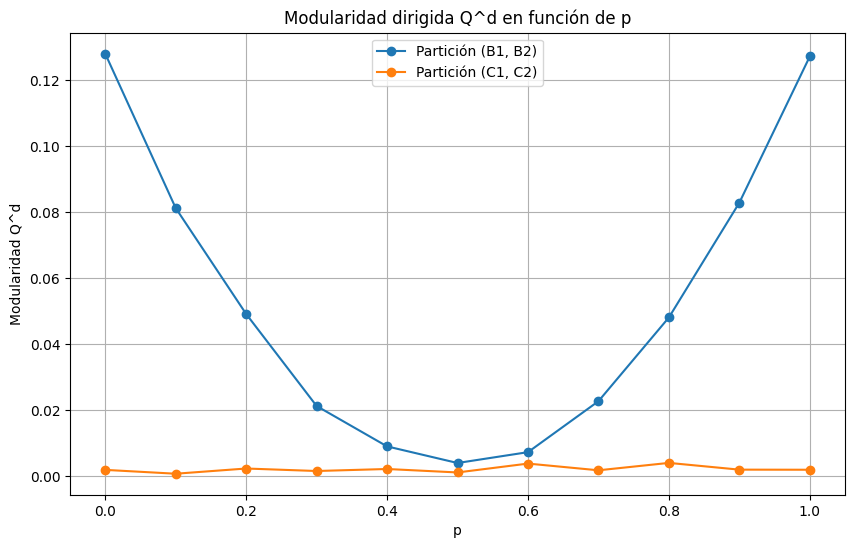
\includegraphics[scale=0.5]{images/modularidad_dirigida.png}
        \caption{Modularidad por particiones en función de $p$}
        \label{fig:grafico_modularidad}
    \end{figure}

    Es posible notar del gráfico que desde $p = 0$ la modularidad de la primera partición, $(B1, B2)$, disminuye a medida que aumenta el valor de $p$ hasta llegar a $p = 0,5$, donde se presenta la menor modularidad del grafo, para luego ir aumentando a medida que aumenta en valor de $p$.

    En cambio, la modularidad de la segunda partición, $(C1, C2)$, se mantiene baja y no varía mucho en comparación a la primera partición, además se puede notar que no sigue un patrón claro en relación a si disminuye/aumenta su valor a medida que aumenta el valor de $p$. 

    Esto nos puede decir que la primera partición es mucho más sensible a la estructura que presenta el grafo, y además se obtienen los mayores valores de modularidad cuando $p = 0$ y $p = 1$, lo que muestra la clara separación entre los nodos de $B1$ y $B2$. Mientras que, para la segunda partición no se puede ver reflejada ninguna estructura del grafo debido a los valores bajos de la modularidad y tampoco varían mucho con los distintos valores de $p$. Todo esto refleja la importancia que tiene la partición elegida en la detección de la estructura de una red.
    
    \item Dado que todos los nodos tienen grado $k$, el grado promedio de la red también es $k$. Dicho esto, queremos que de acuerdo con la teoría de percolación, queremos que se cumpla lo siguiente: $$1-\frac{1}{k} > 0.95$$ $$0.05>\frac{1}{k}$$ $$k>\frac{1}{0.05}$$ $$k>20$$ Entonces, $k$ debe ser mayor a 20 para que al eliminar el 95 \% de los nodos siga existiendo una componente gigante.
    
    \item
    \begin{enumerate}
        \item El gráfico de la red es el siguiente:
        \begin{figure}[H]
            \centering
            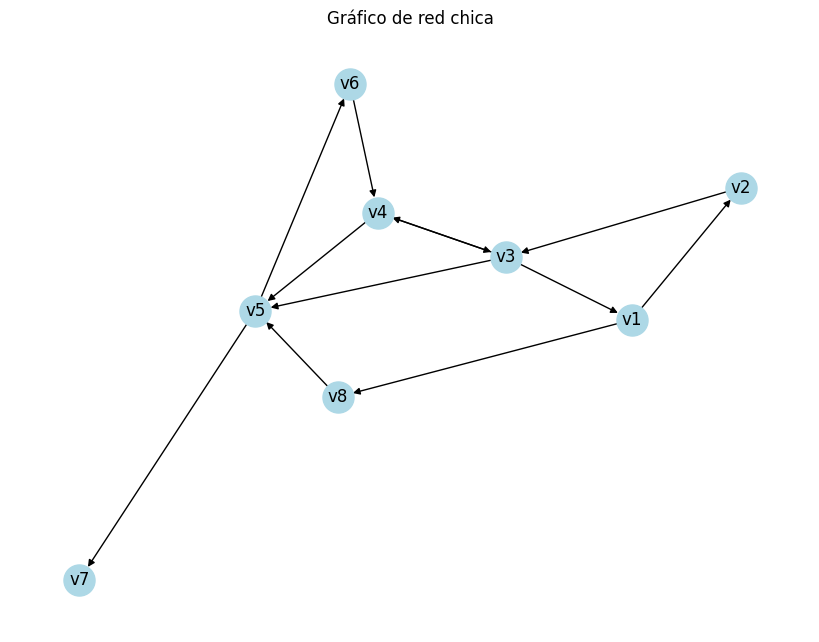
\includegraphics[scale=0.5]{images/grafico_red_chica.png}
            \caption{Gráfico de red chica}
            \label{fig:graph_red_chica}
        \end{figure}

        Los valores del grado de entrada, betweenness y PageRank de cada nodo son:
        
        \begin{table}[H]
            \centering
            \begin{tabular}{|c|c|c|c|}
            \hline
            \textbf{Nodo} & \textbf{Grado de entrada} & \textbf{Betweenness} & \textbf{PageRank} \\ \hline
            v1 & $1$ & $0,238095$ & $0,077725$ \\ \hline
            v2 & $1$ & $0,047619$ & $0,064579$ \\ \hline
            v3 & $2$ & $0,428571$ & $0,162980$ \\ \hline
            v4 & $2$ & $0,309524$ & $0,180098$ \\ \hline
            v5 & $3$ & $0,357143$ & $0,209159$ \\ \hline
            v6 & $1$ & $0,214286$ & $0,120440$ \\ \hline
            v7 & $1$ & $0,000000$ & $0,120440$ \\ \hline
            v8 & $1$ & $0,071429$ & $0,064579$ \\ \hline
            \end{tabular}
            \caption{Valores de grado de entrada, betweenness y PageRank}
            \label{tab:values_red_chica}
        \end{table}

        \item El ranking de los nodos según su grado de entrada sería:
        \begin{enumerate}
            \item v5 ($3$).
            \item v3 y v4 ($2$).
            \item v1, v2, v6, v7 y v8 ($1$).
        \end{enumerate}

        Luego, el ranking de los nodos según su betweenness sería:
        \begin{enumerate}
            \item v3 ($0.428571$).
            \item v5 ($0.357143$).
            \item v4 ($0.309524$).
            \item v1 ($0.238095$).
            \item v6 ($0.214286$).
            \item v8 ($0.071429$).
            \item v2 ($0.047619$).
            \item v7 ($0.000000$).
        \end{enumerate}

        Finalmente, el ranking de los nodos según su valor de PageRank sería:
        \begin{enumerate}
            \item v5 ($0.209159$).
            \item v4 ($0.180098$).
            \item v3 ($0.162980$).
            \item v6 y v7 ($0.120440$).
            \item v1 ($0.077725$).
            \item v2 y v8 ($0.064579$).
        \end{enumerate}

        \item Se puede observar una relación entre grado de entrada, betweenness y valor de PageRank, específicamente para los nodos con altos valores de estos, que es posible notar en los nodos v3, v4 y v5. Se puede decir que los nodos que tienen una mayor cantidad de conexiones de entradas son considerados más importantes en el grafo y, a su vez, son importantes como puente entre otros dos nodos.

        Otro caso interesante es que el nodo v7 tenga un mayor valor de PageRank que los nodos v2 y v8, considerando que su valor de betweenness es 0. Esto se puede deber a que el nodo v7 tiene una conexión de entrada con un nodo con PageRank elevado, en comparación a los nodos v2 y v8 que tienen una conexión de salida con un nodo con PageRank elevado.
    \end{enumerate}
    
    \item Al determinar los motifs de la red, en base a los motifs presentados en las diapositivas de la clase, se obtienen los siguientes resutados:
    
    \begin{table}[H]
        \centering
        \begin{tabular}{|c|c|}
            \hline
            \textbf{Motif} & \textbf{Frecuencia} \\ \hline
            M1 & $0$ \\ \hline
            M2 & $0$ \\ \hline
            M3 & $9767$ \\ \hline
            M4 & $0$ \\ \hline
            M5 & $0$ \\ \hline
            M6 & $0$ \\ \hline
            M7 & $0$ \\ \hline
            M8 & $0$ \\ \hline
            M9 & $0$ \\ \hline
            M10 & $1777$ \\ \hline
            M11 & $0$ \\ \hline
            M12 & $0$ \\ \hline
            M13 & $0$ \\ \hline
        \end{tabular}
        \caption{Frecuencia de los diferentes motifs presentes en la red}
        \label{tab:motifs}
    \end{table}

    Se puede notar como solamente se indentifican dos tipos de motifs en la red M3 y M10. El motif M3 representa una secuencia lineal de citaciones, donde un paper $A$ cita a otro paper $B$, que a su vez este paper $B$ cita a otro paper $C$, tiene una frecuencia de $9767$, lo que tiene sentido en esta red, ya que con el paso del tiempo surgen nuevas formas de representar problemas, ideas y posibles soluciones inspirado en el trabajo previo.
    
    En cambio, el motif M10 representa colaboraciones entre estos papers, donde un paper $A$ y $B$ se citan mutuamente y ambos citan por separado a un paper $C$, este motif tiene una frecuencia de $1777$ lo que sugiere la existencia de comunidades que colaboran estrechamente entre ellos inspirados en algún trabajo previo en común.

    Además, la ausencia de los otros motifs sugiere que se tiene una red considerablemente simple, sin relaciones entre citaciones complejas o muy entrelazadas entre sí.

    Para el cálculo del vector de clustering dirigido propuesto por Ahnert \& Fink se implementó una función que lo calcularía pero, debido a nuestra capacidad computacional, no fue posible ejecutar dicho código exitosamente.
    
    \item A continuación se muestra el gráfico de $p$ versus $d$:
    \begin{figure}[H]
        \centering
        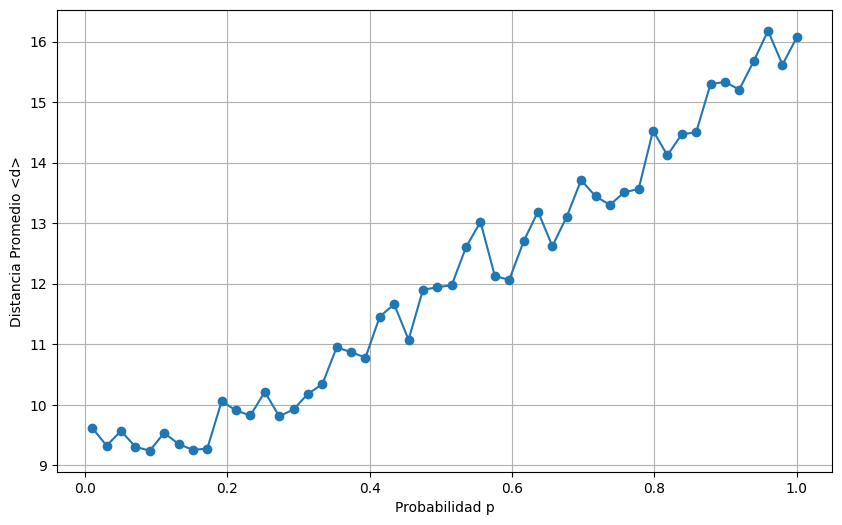
\includegraphics[scale=0.5]{images/grafico_p8.png}
        \caption{Relación entre $p$ y distancia promedio}
        \label{fig:graph_p}
    \end{figure}
    Se puede observar que mientras mayor sea la probabilidad $p$ (es decir, $1-p$ es menor), mayor es la distancia promedio. Sin embargo, no se observa un claro cambio de fase entre un mundo grande y un mundo pequeño. Esto puede deberse a que n no es lo suficientemente grande, por lo que sería interesante intentarlo con una mayor cantidad de nodos.
\end{enumerate}


\end{document}